    %   Il progetto nasce dal template per il frontespizio realizzato da Marco Antonio Corallo, che ringrazio. Seguono alcuni commenti per evidenziare la presenza di alcuni pacchetti che mi sono stati utili per la stesura della tesi. Chiaramente, dipende tutto dal tipo di lavoro che uno vuole eseguire, che determina anche le diverse esigenze. Durante la stesura ho passato molto tempo su siti e forum a cercare di risolvere alcuni probelmi di formattazione, ma in generale Latex è stato piuttosto versatile. 

% Tipo di documento. L'uso di twoside implica che i capitoli inizino sempre con la prima pagina a sinistra, eventualmente lasciando una pagina vuota nel capitolo precedente. Se questa cosa è fastidiosa, è possibile rimuoverlo. 
\documentclass[a4paper, twoside,openright]{report}

% Dimensione dei margini
\usepackage[a4paper,top=3cm,bottom=3cm,left=3cm,right=3cm]{geometry} 
% removes this restriction by allowing font sizes at arbitrary sizes
\usepackage{lmodern}
% Dimensione del font
\usepackage[fontsize=13pt]{scrextend}
% Lingua del testo
\usepackage[english]{babel} % ,italian
% Lingua per la bibliografia
\usepackage[fixlanguage]{babelbib}
% pacchetto per la bibliografia
%Includes "References" in the table of contents
\usepackage[nottoc]{tocbibind}
% pacchetto natbib per la bibligrafia in formato autore-anno
\usepackage[round]{natbib} 
% \usepackage{biblatex}
% Codifica del testo
\usepackage[utf8]{inputenc} 
% Encoding del testo
\usepackage[T1]{fontenc}
% Permette di generare testo fittizio. Mi è stato utile 
% per capire quale sarebbe stata l'impostazione del 
% testo nella pagina prima che scrivessi un determinato paragrafo
\usepackage{lipsum}
% Per ruotare le immagini
\usepackage{rotating}
% Per modificare l'header delle pagine 
\usepackage{fancyhdr}               

% Librerie matematiche
% \usepackage{amssymb}
\usepackage{amsmath}
\usepackage{amsthm}         

% Uso delle immagini
\usepackage{graphicx}
% Uso dei colori
\usepackage[dvipsnames]{xcolor}         
% Uso dei listing per il codice
\usepackage{listings}          
% Per inserire gli hyperlinks tra i vari elementi del testo 
\usepackage{hyperref}     
% Diversi tipi di sottolineature
\usepackage[normalem]{ulem}

% -----------------------------------------------------------------

% Modifica lo stile dell'header
\pagestyle{fancy}
\fancyhf{}
\lhead{\rightmark}
\rhead{\textbf{\thepage}}
\fancyfoot{}
\setlength{\headheight}{12.5pt}

% Rimuove il numero di pagina all'inizio dei capitoli
\fancypagestyle{plain}{
  \fancyfoot{}
  \fancyhead{}
  \renewcommand{\headrulewidth}{0pt}
}

% Stile del codice
\lstdefinestyle{codeStyle}{
    % Colore dei commenti
    commentstyle=\color{teal},
    % Colore delle keyword
    keywordstyle=\color{Magenta},
    % Stile dei numeri di riga
    numberstyle=\tiny\color{gray},
    % Colore delle stringhe
    stringstyle=\color{violet},
    % Dimensione e stile del testo
    basicstyle=\ttfamily\footnotesize,
    % newline solo ai whitespaces
    breakatwhitespace=false,     
    % newline si/no
    breaklines=true,                 
    % Posizione della caption, top/bottom 
    captionpos=b,                    
    % Mantiene gli spazi nel codice, utile per l'indentazione
    keepspaces=true,                 
    % Dove visualizzare i numeri di linea
    numbers=left,                    
    % Distanza tra i numeri di linea
    numbersep=5pt,                  
    % Mostra gli spazi bianchi o meno
    showspaces=false,                
    % Mostra gli spazi bianchi nelle stringhe
    showstringspaces=false,
    % Mostra i tab
    showtabs=false,
    % Dimensione dei tab
    tabsize=2
} \lstset{style=codeStyle}

% Stile di codice per dimensioni maggiori, in cui ho avuto bisogno di un testo più picolo (ad esempio se si vuole inserire del codice che ha linee molto lunghe). Per usare questo stile piuttosto che il precedente, usare 

% \lstset{style=longBlock}
%  % inserire il codice...
% \lstset{style=codeStyle}

% Il secondo comando consente di tornare allo stile precedente 
\lstdefinestyle{longBlock}{
    commentstyle=\color{teal},
    keywordstyle=\color{Magenta},
    numberstyle=\tiny\color{gray},
    stringstyle=\color{violet},
    basicstyle=\ttfamily\scriptsize,
    breakatwhitespace=false,         
    breaklines=true,                 
    captionpos=b,                    
    keepspaces=true,                 
    numbers=left,                    
    numbersep=5pt,                  
    showspaces=false,                
    showstringspaces=false,
    showtabs=false,                  
    tabsize=2
} \lstset{style=codeStyle}

% si inseriscono nella bibliografia anche le fonti presenti in Bibliography.bib ma non citati direttamente con il comando \cite
\nocite{*}

% Margini prima e dopo blocchi di codice, per avere più distanza
\lstset{aboveskip=20pt,belowskip=20pt}

% Modifica dello stile dei riferimenti, con il testo in cyano
\hypersetup{
    colorlinks,
    linkcolor=CornflowerBlue,
    citecolor=CornflowerBlue
}

% Aggiunti definizioni, teoremi, linea e listing
\newtheorem{definition}{Definizione}[section]
\newtheorem{theorem}{Teorema}[section]
\providecommand*\definitionautorefname{Definizione}
\providecommand*\theoremautorefname{Teorema}
\providecommand*{\listingautorefname}{Listing}
\providecommand*\lstnumberautorefname{Linea}

\raggedbottom

%\newcommand{\cgs}[1]{{\textcolor{brown}[\textcolor{red}{\bf{GS: }}{ \textcolor{brown}{#1]}}}}             
%\newcommand{\cmc}[1]{{\textcolor{blue}[\textcolor{magenta}{\bf{MC: }}{ \textcolor{blue}{#1]}}}}



% -----------------------------------------------------------------
\begin{document}

\begin{titlepage}
\begin{figure}[!htb]
    \centering
    
\includegraphics[keepaspectratio=true,scale=0.5]{images/Frontespizio/cherubinFrontespizio.eps}
\end{figure}

\begin{center}
    \LARGE{UNIVERSITÀ DI PISA}
    \vspace{5mm}
    \\ \large{DIPARTIMENTO DI INGEGNERIA DELL'INFORMAZIONE}
    \vspace{5mm}
    \\ \LARGE{Laurea Triennale in Ingegneria Informatica}
\end{center}

\vspace{15mm}
\begin{center}
    {\LARGE{\bf Un fantastico titolo\\ \vspace{5mm} per la mia tesi di laurea! }}
    
    % Se il titolo è abbastanza corto da stare su una riga, si può usare
    
    % {\LARGE{\bf Un fantastico titolo per la mia tesi!}}
\end{center}
\vspace{30mm}

\begin{minipage}[t]{0.47\textwidth}
	{\large{Relatore:}{\normalsize\vspace{3mm}
	\bf\\ \large{Prof: Nome Cognome} \normalsize\vspace{3mm}\bf \\ \large{Prof: Nome Cognome}}}
\end{minipage}
\hfill
\begin{minipage}[t]{0.47\textwidth}\raggedleft
	{\large{Candidato:}{\normalsize\vspace{3mm} \bf\\ \large{Nome Cognome}}}
\end{minipage}

\vspace{30mm}
\hrulefill
\\\centering{\large{ANNO ACCADEMICO 202X/202Y}}

\end{titlepage}
% todo: blank page after titlepage

\normalsize
Modern language models based on deep artificial neural networks have achieved significant progress in Natural Language Processing applications. This has spawned a line of research aimed at clarifying which linguistic phenomena and generalizations are actually learned by these models. One of the main approaches for this goal, is testing these models' sentence acceptability estimates with fine-grained targeted linguistic evaluations, based on minimal pairs that isolate a particular linguistic phenomenon.\\

This kind of assessment is relevant to address the open problems of the limitations that these models still have, like being significantly data-inefficient in their training, compared to humans’ language acquisition and learning skills; or their still insufficient linguistic performance or generalization for some linguistic phenomena. This kind of assessment has also a broad interdisciplinary relevance since language models could be used to test theoretical linguistics hypotheses, and theoretical linguistics and psycholinguistics could in turn provide insights on how to improve these models' linguistic skills to more human-like levels.\\ 

In this work, we focus on the syntactic phenomena of island effects, and extend the Italian test suite from the psycholinguistic and experimental syntax work by Sprouse et al. (2016). Then,  we evaluate on these test suites two transformer-based language models (Gpt-2 and Bert), pretrained in Italian, and compare their performance with those on humans. We propose that our adaptation of the factorial test design by Sprouse et al. could be complementary to benchmarks like BLiMP (Warstadt et al. 2020) which are based on minimal pairs tests, and allows to test more aspects of linguistic phenomena like extraction islands.

 %% Hello! this is the sourcecode!

\tableofcontents

% Rimuovere se non si vuole la tabella delle figure
\listoffigures

\chapter{Questo è un capitolo}

\lipsum[1]

\section{Questa è una sezione}

\lipsum[2]

\subsection{Questa è una sottosezione}

\lipsum[3]

\subsubsection{Questa è una sotto-sottosezione}

\lipsum[4]

É possibile riferire l'immagine, una volta assegnatagli una label, tramite il comando \texttt{\textbackslash autoref\{fig:immagine\}}, ottenendo il seguente risultato: \autoref{fig:immagine}.

\begin{figure}
    \centering
    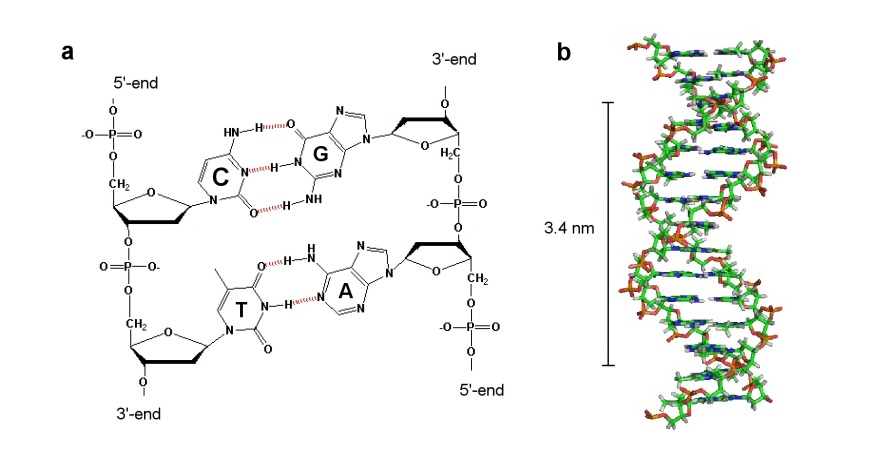
\includegraphics[width=0.8\textwidth]{images/Chapter1/immagine.jpg} % width= 0.8\textwidth
    \caption{Questa è un'immagine} 
    \label{fig:immagine} % this internally labels the figure for future referencing.
\end{figure}

Questa è una citazione \cite{warstadt2020blimp}.
Questa è una citazione "regular in text citation" \citet{warstadt2020blimp}.  % or \cite{<key>}
Questa è una citazione tra parentesi \citep{warstadt2020blimp}
Questa è un'altra citazione \citep{wei2021frequency}
Listing bibliography entries \citep{hu2020systematic, lau2020furiously,  sprouse2016experimental}

\subsubsection{Questa è un'altra sottosezionelipsum}

Quello che segue è un esempio di codice. E' possibile modificare il linguaggio per il synyax highlight, aggiungere parole chiave... E' tutto disponibile nella guida del pacchetto \texttt{listings}.

\lstinputlisting[language=C++]{listings/Capitolo1/code1.cpp} 

\section{Misc notes with refs}

“NATURAL LANGUAGE DOES NOT MAXIMIZE PROBABILITY” 
“Why is human-written text not the most probable text? We conjecture that this is an intrinsic property of human language. Language models that assign probabilities one word at a time without a global model of the text will have trouble capturing this effect. Grice’s Maxims of Communication (Grice, 1975) show that people optimize against stating the obvious. Thus, making every word as predictable as possible will be disfavored. This makes solving the problem simply by training larger models or improving neural architectures using standard per-word learning objectives unlikely: such models are forced to favor the lowest common denominator, rather than informative language.” 
\citep{holtzman2019curious}

Repeated exposure to a type of island construct will increase its perceived acceptability 
\citep{chaves2014subject}

Targed ..syntactic tests on modern language models seem to have started with \citet{linzen2016assessing}, while the use of psycholinguistic tests for this seem to have started with \citet{futrell2018rnns}.

\subsection{Sottosezione con una tabella}

La tabella si indirizza sempre con l'uso di una label, ottenendo il risultato \autoref{tab:labelTabella}.

\begin{table}
    \caption{Una simpatica tabella!}\label{tab:labelTabella}
    \begin{center}
    \begin{tabular}{c|c|c|c}
        \textbf{Colonna 1} & \textbf{Colonna 2} & \textbf{Colonna 3} & \textbf{Colonna 4} \\
        \hline
            $3$      & $24$     & $24$    & $29$ \\ 
            $36$     & $31$     & $49$    & $39$ \\ 
            $32$     & $41$     & $59$    & $57$ \\ 
            $34$     & $60$     & $79$    & $74$ \\ 
            $328$    & $96$     & $194$   & $99$ \\ 
            $356$    & $117$    & $297$   & $149$ \\ 
            $312$    & $315$    & $293$   & $242$ \\ 
            $3024$   & $184$    & $253$   & $019$ \\ 
            $3048$   & $7795$   & $253$   & $077$ \\ 
            $3096$   & $7767$   & $2432$  & $0514$ \\ 
            $3192$   & $3769$   & $2435$  & $0551$ \\ 
            $36384$  & $6625$   & $3432$  & $0497$ \\ 
            $32768$  & $15469$  & $6472$  & $0471$ \\ 
            $35536$  & $15425$  & $14539$ & $10289$ \\ 
            $331072$ & $34623$  & $24941$ & $20444$ \\  
        \end{tabular}
    \end{center}
\end{table}

\appendix

\chapter{Factorial design plots}

..

\section*{Questa è un'altra sezione, ma non viene inserita nell'indice}

..


\bibliographystyle{plainnat} 
\bibliography{chapters/Bibliografia}


% .. 
% \addbibresource{references.bib}
% \include{chapters/Bibliografia}
\end{document}
% -----------------------------------------------------------------
